% Public development manuscript; no submission or independent validation claim.
\documentclass[10pt,twocolumn,letterpaper]{article}
\usepackage[T1]{fontenc}
\usepackage[pagenumbers]{cvpr}
\usepackage{microtype}
\usepackage{tabularx}
\definecolor{cvprblue}{rgb}{0.15,0.43,0.64}
\usepackage[pagebackref,breaklinks,colorlinks,allcolors=cvprblue]{hyperref}
\def\confName{CVPR}
\def\confYear{2026}
\makeatletter
\newcommand{\tableinput}[1]{\@@input #1 }
\makeatother
\title{BrickAtlas Hierarchy: Crossed Evaluation of\\
Brick Structure, Reasoning, and Executable Intervention}
\author{Development Manuscript\\Author and affiliation metadata intentionally omitted}
\begin{document}
\input{hierarchy-expanded-results.tex}
\maketitle

\begin{abstract}
Understanding an assembly requires more than recognizing its parts:
an agent must reason about dependencies, identify missing information,
and execute interventions without violating intermediate constraints.
We introduce BrickAtlas Hierarchy, a benchmark that holds object identity
fixed while varying these requirements. The Hierarchy-3 release crosses
144 authored digital configurations with 48 shared task families,
yielding 6,912 questions on 42,617 visible primitives. Four structural
strata each contain 36 configurations; every configuration supports
22 atomic, 15 metacognitive/physical, six procedural, and five integrative
tasks. A public state-transition interpreter validates action sequences,
while resource and possible-world contracts check schedules and policies.
Rapier supplies collision queries and sampled dynamic observations.
The same model records and interpreter drive interactive 3D inspection
and replay. All 6,912 reference answers satisfy their contracts, and
a solver using public preconditions solves all 1,152 action tasks.
A historical GPT-4.1 mini pilot achieves 7/16 exact successes; its
error decomposition separates interface failures from reasoning errors.
These controls establish inspectable execution, while the small pilot,
shared constructors, and uncalibrated physics limit performance and
real-world claims.
\end{abstract}

\begin{figure*}[t]
\centering
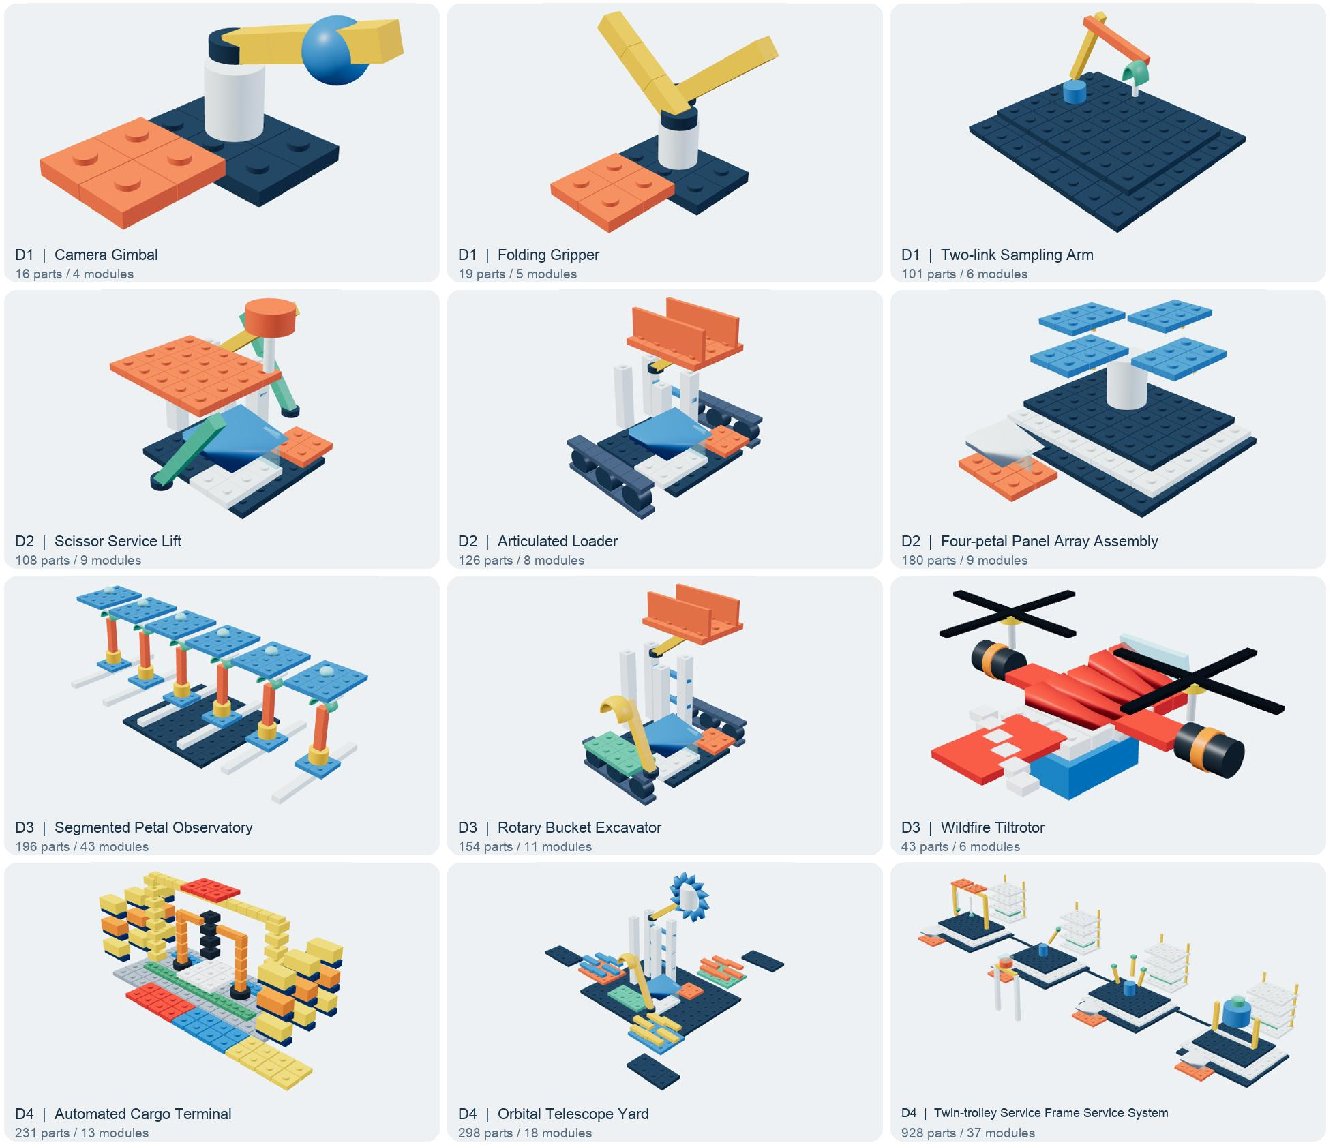
\includegraphics[width=.96\textwidth]{figures/publication-teaser.pdf}
\caption{\textbf{Representative configurations across structural strata.}
Rows progress from D1 components to D4 systems. All panels are actual
3D canvas renders. The release includes 144 configurations, and the
supplement provides four views and a task index for every configuration.
Part count and structural scope need not increase together.}
\label{fig:objects}
\end{figure*}

\section{Introduction}
An agent can identify a gripper yet remove its supporting module too
early. It can propose the correct replacement but omit verification,
or select a useful inspection without specifying what to do after
each possible observation. Such failures couple structural understanding
with sequential and conditional reasoning. A final correct-looking
object does not establish that an intervention respected its constraints.

Digital brick environments offer discrete identities, hierarchical
assemblies, and reproducible edits. Recent work studies generative
assembly~\cite{pun2025brickgpt,kulits2026bricknet}, interactive
reconstruction~\cite{walsman2022break}, and physical
planning~\cite{ma2025phyblock}. These settings motivate a complementary
question: how can evaluation separate the effect of object structure
from the effect of the task requested on that object?

BrickAtlas crosses two axes. The structural axis ranges from D1 local
components through D2 assemblies and D3 mechanisms to D4 systems.
The task axis ranges from atomic questions to metacognitive/physical
reasoning, executable procedures, and integrated constraints. All
48 task families occur on every configuration. This supports comparisons
across levels at fixed task identity and across tasks at fixed object
identity. The axes specify coverage, not an assumption that every
higher-level question is empirically harder.

Three choices make failures inspectable. First, physics-derived questions
refer to archived simulator observations. Second, a submitted procedure
executes a public state machine, so independent legal actions can commute
without matching one canonical answer string. Third, intermediate
states are rendered by the original 3D application using the same
interpreter as scoring. A rejected transition can thus be inspected
alongside its missing precondition and unchanged geometry.

The release contains 144 configurations and 6,912 questions. Its
authored, reusable constructors allow systematic coverage but create
correlated examples. We distinguish configurations, geometry fingerprints,
task instances, and views throughout. The public development set
contains no hidden confirmation split. OMR/LDraw examples inform visual
design but are not benchmark cases.

Our contributions are:
\begin{enumerate}
\item a complete configuration-by-task design with four structural
strata and 48 families repeated on every object;
\item executable action, resource-schedule, and possible-world contracts
that expose intermediate failures and information requirements;
\item a reproducible 3D release with 576 canonical views and shared
scoring/replay semantics; and
\item data-derived structural statistics, answer-distribution controls,
physical audit results, and a bounded historical model diagnostic.
\end{enumerate}

\section{Related Work}
\paragraph{Generation and structural validity.}
BrickGPT~\cite{pun2025brickgpt} addresses stable brick generation.
BrickNet~\cite{kulits2026bricknet} represents assembly with typed
connection graphs and evaluates connectivity and collisions using
valid-prefix length. It reports 320,808 pretraining samples and 67,185
supervised fine-tuning samples; these are training-sample counts,
not independent source-object counts. BrECS~\cite{ahn2024brecs}
studies sequential assembly under a budget. BrickAtlas fixes the
configuration and varies questions and interventions; it does not
introduce a competing generator or claim comparable asset scale.

\paragraph{Reasoning and construction plans.}
LEGO-Puzzles~\cite{tang2025legopuzzles} studies multistep spatial
reasoning. PhyBlock~\cite{ma2025phyblock} contains 400 assembly tasks
and 2,200 VQA tasks, using Genesis and progressive planning
requirements. Manual-based methods such as MEPNet~\cite{wang2022manual},
Neural Assembler~\cite{yan2024assembler}, and
TreeSBA~\cite{guo2024treesba} recover poses or construction steps.
Our contribution is the shared task-by-configuration organization
with executable contracts, rather than novelty of every task family.

\paragraph{Disassembly and embodiment.}
Break and Make~\cite{walsman2022break} requires inspection and
disassembly followed by reconstruction from an empty scene in LTRON.
Its source collection includes 1,727 OMR files; evaluation includes
part, pose, and edge agreement and assembly edit distance.
Our dismantling task is a dependency contract over rigid modules,
and does not reproduce that visual exploration problem.
WorkBenchMark~\cite{ma2026workbenchmark} and
BC-Bench~\cite{liu2026composer} address embodied or compositional
assembly. We separate digital state validity from insertion force,
connector tolerances, grasping, and hardware transfer.

\begin{table*}[t]
\centering\small
\begin{tabularx}{\textwidth}{lXXX}
\toprule Setting & Input and objective & Primary evidence & Relation to BrickAtlas\\\midrule
BrickNet & Conditional generation of brick assemblies & Graph connectivity and collision prefixes & Validity of a generated structure\\
Break and Make & Inspect, dismantle, then reconstruct & Interactive observations and assembly agreement & Reconstruction after exploration\\
PhyBlock & Physical questions and assembly planning & VQA answers and simulated assembly & Progressive physical planning\\
BrickAtlas & Fixed configuration, 48 repeated task families & Choices, transition traces, schedules, policies & Matched reasoning and intervention contracts\\
\bottomrule
\end{tabularx}
\caption{Comparison of evaluation settings, not a performance comparison.
Different source units, information conditions, and validators prevent
directly pooling reported dataset sizes or scores.}
\label{tab:related}
\end{table*}

\section{Library and Crossed Design}
\subsection{Representation}
A model consists of parts $\mathcal P$, rigid modules $\mathcal M$,
and declared joints $\mathcal J$. Each part records shape, dimensions,
local pose, color, and module membership. Each module records world
pose, mass, role, and anchoring status. Each joint records endpoints,
local anchors, type, axis, and limits. Parent-to-child joint directions
induce an assembly dependency order, while support queries use
undirected connectivity to anchored roots.

The visible vocabulary includes bricks, plates, beams, windows,
slopes, arches, cylinders, wheels, axles, gears, and spheres. These
are LEGO-like digital primitives, not verified commercial part
specifications. A procedure operates on rigid modules; it does not
necessarily separate every visible primitive.

\subsection{Structural Coverage and Provenance}
D1 contains local devices such as gimbals, grippers, hatches, and
valve stands. D2 introduces complete assemblies such as service lifts,
loaders, trackers, and inspection craft. D3 contains articulated
mechanisms including cranes, observatories, robots, and excavators.
D4 combines multiple workcells in cargo terminals, docking yards,
energy stations, and service hangars (Fig.~\ref{fig:objects}).

\begin{table}[t]
\centering\small
\setlength{\tabcolsep}{3pt}
\begin{tabular}{lrrrrrr}
\toprule & & \multicolumn{2}{c}{Parts/layout} & & & \\
Level & $N$ & Range & Median & Modules & Depth & Tasks\\\midrule
\tableinput{tables/publication-structure.tex}
\bottomrule
\end{tabular}
\caption{Measured structural coverage. Modules and dependency depth
are min--max ranges. Depth counts nodes on a longest root-to-module path.}
\label{tab:scale}
\end{table}

Table~\ref{tab:scale} reports measured sizes. The collection contains
42,617 parts, 2,040 modules, and 1,938 joints. D2 and D3 overlap in
part count because strata describe structural scope rather than
psychometrically calibrated difficulty. Local questions may remain
easy even in a large scene when the relevant attributes are explicit.

All configurations are agent-authored from reusable construction
primitives; no independent human design study was conducted. The
release retains 48 corrected configurations and their 2,304 tasks
byte-for-byte, adding 96 configurations and 4,608 tasks. Twelve added
constructor families contribute two configurations at each of four
levels. They include arms, grippers, carousels, cross-feed stages,
cradles, drums, gantries, folding panels, elastic suspensions, gates,
inclined probes, and turntables.

The 96 additions have distinct geometry fingerprints after removing
names, colors, and global translation. A retained latch and probe
stage share geometry with different joints, giving 143 geometry
fingerprints overall. Constructor reuse still creates dependence
among geometrically distinct layouts. Future train/test partitions
must group shared constructors and lineage, not randomly split
individual questions. The retired procedural-grid sources are
excluded from current counts.

\subsection{Matched Task Coverage}
\begin{table*}[t]
\centering\small
\begin{tabularx}{\textwidth}{lrrrX}
\toprule Task layer & Families & Per level & Total & Representative requirements\\\midrule
Atomic & 22 & 792 & 3,168 & Identify, count, edit an attribute, infer topology, transform coordinates.\\
Meta / physical & 15 & 540 & 2,160 & Diagnose, interpret physical records, inspect, abstain, minimize expected loss.\\
Procedural & 6 & 216 & 864 & Assemble, dismantle, repair, compound edit, guarded repair, rollback.\\
Integrative & 5 & 180 & 720 & Repair multiple faults, share tools, schedule, choose conditional policies.\\\midrule
Total & 48 & 1,728 & 6,912 & All 48 families occur on each configuration; each level has 36 configurations.\\
\bottomrule
\end{tabularx}
\caption{Crossed evaluation design. Task layers describe composition;
D1--D4 describe object structure. The supplement enumerates all families.}
\label{tab:taxonomy}
\end{table*}
Table~\ref{tab:taxonomy} defines the crossing. Task IDs bind configuration
and family. Another render, color, answer order, or fault condition
does not create a new source object. The 6,912 outputs comprise
4,608 single choices, 720 choice sets, 1,152 action programs,
144 schedules, and 288 policies. Procedural tasks and two integrative
families share the action-program format; task layer and output
format are distinct annotations.

\section{Task and Scoring Contracts}
A task is $t=(m,f,x,\mathcal Y,V)$: configuration $m$, family $f$,
public evidence $x$, output space $\mathcal Y$, and deterministic
validator $V$. An inference input contains canonical image evidence
and the task-specific public record, excluding the reference answer.
The browser exposes reference answers for audit and is therefore
separate from the blinded input export.

\subsection{Atomic and Metacognitive Questions}
Atomic tasks return a choice ID. Distractors vary a relevant attribute,
identity, count, set, or transformation. Option order rotates
deterministically per task. Set-valued alternatives are canonicalized
before deduplication; vectors and programs remain ordered. Some
questions have fewer than four distinct alternatives, so chance
baselines must use the actual option count.

Multiple-choice tasks require the complete feasible set. Accessibility
can have an empty feasible set when every candidate path collides.
Counterfactual support removes a specified module, excludes it from
the answer, and recomputes reachability to any anchored root through
remaining joint edges. Redundant support paths are allowed.

The base inspection family uses a uniform finite prior and deterministic
observations. For query $q$ with observation groups of size $n_o$
among $N$ worlds and cost $c(q)$, utility is
\begin{equation}
U(q)=\frac{-\sum_o (n_o/N)\log_2(n_o/N)}{c(q)}.
\end{equation}
All maximizing queries are accepted. Abstention tests whether compatible
worlds imply the same action. Posterior questions condition the prior
on an observation; weighted-posterior questions supply nonuniform
weights. Expected-loss questions select an action minimizing
$\sum_w p(w)\ell(a,w)$. Pareto questions enumerate every non-dominated
cost/mass/stiffness alternative. Force-moment questions use explicit
lever arms and forces; physical-trace questions read simulator records.

Most atomic public records disclose structural attributes needed to
solve the task. Their scores therefore measure structured reasoning
with auxiliary images, not isolated visual perception. Image-removal,
symbolic-removal, and viewpoint ablations are required before claiming
visual reasoning gains. English examples in this paper translate
the task intent; the released prompts retain their original language,
which must be reported in future experiments.

\subsection{Executable Procedures}
An action is $a=(P_a,F_a,A_a,D_a,c_a)$: required facts, forbidden facts,
add effects, delete effects, and cost. Execution from state $S$
requires $P_a\subseteq S$ and $F_a\cap S=\varnothing$, followed by
\begin{equation}
S'=(S\setminus D_a)\cup A_a.
\end{equation}
The interpreter processes submitted IDs in order and stops at the
first unknown action, failed precondition, forbidden state, or budget
overrun. Success additionally requires all positive terminal goals
and the absence of any prohibited terminal facts. A legal incomplete
prefix is not a successful procedure.

Assembly places modules after their declared predecessors. Disassembly
removes children before parents. Service repair requires support,
opening, removal, replacement, verification, closure, and release.
Compound editing substitutes a protected color operation. Guarded
repair and rollback expose unsafe shortcuts; exclusive-tool repair
removes a shared availability fact until the current intervention
releases it. Independent actions may commute, so scoring checks
states rather than equality with a reference list.

\begin{figure*}[t]
\centering
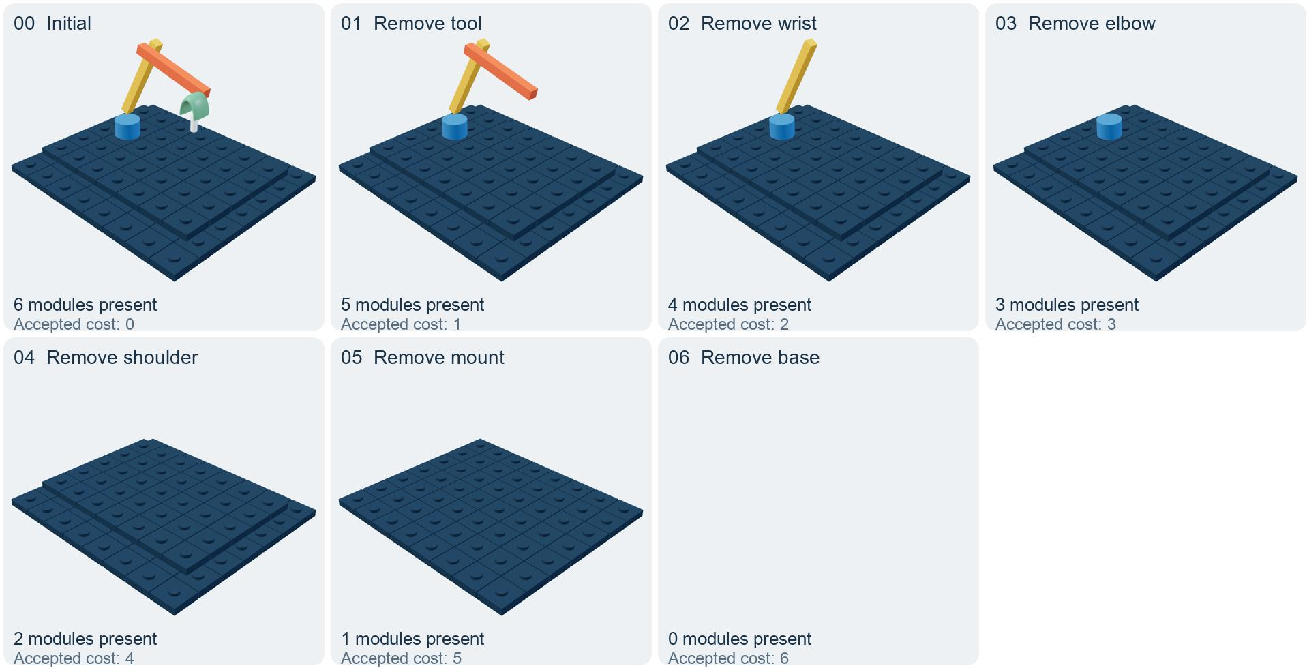
\includegraphics[width=\textwidth]{figures/publication-disassembly.pdf}
\caption{\textbf{Complete dependency-respecting dismantling.}
Actual replay of \texttt{exp-d1-arm-2}: remove tool, wrist, elbow,
shoulder, mount, then foundation. Each panel is the state after the
named action, using identical crop and scale. The final panel is
empty because all six modules were removed. These are symbolic
removals, not continuous extraction trajectories.}
\label{fig:disassembly}
\end{figure*}

\subsection{From Local Reasoning to Dismantling}
Figure~\ref{fig:disassembly} illustrates how the layers relate.
Initially, the atomic \texttt{remove} family asks which module is a
leaf; \texttt{parent} and \texttt{degree} query the same graph.
Each disassembly action requires all children of its target to be
absent. Removing the foundation first fails at step one. The
\texttt{prefix} family tests analogous predecessor reasoning on
assembly sequences, while \texttt{counterfactual} separately asks
which modules lose anchored connectivity after a specified removal.
These are separate tasks on a shared object, not additional questions
counted for each replay frame.

The six-node chain takes six actions to dismantle. Repairing its
terminal tool instead takes seven: support, open, remove, replace,
verify, close, release. Verification deletes the fault fact; release
establishes the repaired goal. Support and closure are symbolic
facts and need not change rendered geometry. The supplement gives
every repair state and the exact precondition/effect mapping.

The same interpreter controls module visibility and color in the
website. Symbolic acceptance certifies the intervention contract;
it does not simulate robot motion or physical tool contact for every
action. Exploded layouts are display transformations only.

\subsection{Integrated Constraints}
Distributed repair combines several targets under one budget and final
goal. Scheduling requires nonnegative integer start times, predecessor
completion, non-overlapping use of exclusive resources, and completion
by a deadline. An inspection policy selects one query and maps every
possible observation to an action. Validation checks all compatible
worlds, not only one sampled branch, and enforces the query budget.

No LLM judge determines correctness. Empty or malformed responses
remain failures. Batch scoring retains missing cases in the frozen
denominator and rejects unknown or duplicate case IDs.
For level $d$ and family $f$, the primary score is
\begin{equation}
A_{df}=\frac{1}{|M_d|}\sum_{m\in M_d}V(t_{mf},\hat y_{mf}).
\end{equation}
Report the $4\times48$ matrix before layer and overall averages.
For procedures, also report accepted-prefix length, first failure
cause, terminal goal satisfaction, and cost. Prefix length rewards
legal incomplete programs and cannot replace exact success.
A future model study should freeze cases and information conditions
before inference and resample constructor families for uncertainty
estimates. The present pilot is too small to support those estimates.

\section{Physics and Quality Protocol}
Rapier 0.20.0 runs at 120\,Hz with 64 solver iterations.
Stud-inclusive cuboids conservatively approximate visible parts,
which form compound rigid modules. Fixed, revolute, prismatic, and
spring descriptors instantiate the declared mechanism. Bases are
anchored. Force-based holding motors use stiffness 60,000, damping
1,500, and maximum force 20,000 in scene units.

After 120 nominal steps, the audit measures geometric representative
point displacement, angular displacement, and non-spring joint
residuals. All 144 configurations satisfy thresholds of 0.35 scene
units, 0.15 radians, and 0.02 scene units. Their maxima are 0.05305,
0.01825, and 0.000815 respectively (rounded upward).
Every rendered vertex lies within its envelope. Initial joint anchors
coincide. Oriented-cuboid queries find no inter-module penetration
above 0.005, including at directly joined interfaces. Joint contacts
remain enabled; revolute limits are set and read back, with a driven
over-limit regression control.

A separate static world performs three continuous service shape casts
per object, excluding the serviced module. An off-center impulse
is then followed by 120 dynamic steps and eleven sampled observations.
The impulse and displacement use the same geometric representative
point, preserving the response under changes of local origin.
Dynamic tasks ask for the maximum of the \emph{sampled translational
response}; they do not estimate a continuous peak, rotational safety
bound, or calibrated load threshold.

Finite-force servos and fixed foundations limit the meaning of nominal
success. Cuboid contact validity does not establish commercial LEGO
connector fit, passive stability, arbitrary motion, or insertion
feasibility. Other checks cover identities, finite poses, positive
dimensions, dependency order, image hashes, and website/data parity.
The supplement records exact protocol settings and historical corrections.

\section{Validation and Diagnostic Results}
\subsection{Deterministic Controls}
\begin{table}[t]
\centering\small
\setlength{\tabcolsep}{3pt}
\begin{tabular}{lrrrrr}
\toprule & Choice & Constant & \multicolumn{2}{c}{Choice success (\%)} & Action\\
Level & tasks & passes & Constant & Uniform & length\\\midrule
\tableinput{tables/publication-controls.tex}
\bottomrule
\end{tabular}
\caption{Measured constant-A / empty-set control and analytic uniform
choice expectation. Percentages use only choice tasks. Action length
is the min--max reference-program length across action families.}
\label{tab:controls}
\end{table}
All 6,912 public reference answers satisfy their validators. A
separate solver reading public preconditions, rather than reference
programs, solves all 1,152 action tasks. These are evaluator and
construction checks, not learned visual-model scores; they also
expose the information supplied by the symbolic input.

Table~\ref{tab:controls} separates choice-only and full-set denominators.
Always selecting A for single choices and the empty set for multiple
choices succeeds on 1,340/5,328 choice tasks (25.15\%). Empty
outputs on other contracts give 1,340/6,912 overall (19.39\%).
Uniform guessing has expectation $1/k$ for a single choice with $k$
options and $2^{-k}$ for uniform subset selection. Varying option
counts prevent a universal 25\% chance baseline.

Semantic-majority frequencies measure the most frequent answer value
per family after discarding option letters. They diagnose public-set
answer concentration, not held-out performance. Balanced letters
alone cannot rule out a constant semantic shortcut. The supplement
reports every family's frequency and action length where applicable.
For example, the public majority is 100\% for \texttt{no-op},
90.97\% for \texttt{degree}, and 83.33\% for \texttt{anchor}.
Thus some atomic families currently function as compliance controls
and have limited discriminative value; crossing them with larger
objects does not resolve their answer concentration.

\subsection{Historical Model Pilot}
\begin{table}[t]
\centering\small
\begin{tabular}{lrrrr}
\toprule Level & Atomic & Meta & Procedure & Integrated\\\midrule
\tableinput{tables/hierarchy3-pilot.tex}
\bottomrule
\end{tabular}
\caption{Historical GPT-4.1 mini pilot on retained configurations.
Every cell contains one fixed question; values are exact counts,
not estimates of whole-cell accuracy.}
\label{tab:pilot}
\end{table}
The fixed base-48 pilot selected local-frame transformation,
expected loss, guarded repair, and resource repair at each level.
GPT-4.1 mini received one image and public structured evidence at
temperature zero, with a 2,200-token output cap, no automatic retries,
and no provider fallback. The 16 responses yield seven exact
successes at a recorded cost of \$\PilotCost.
Raw predictions, public-input hashes, provider IDs, and costs are
archived. No new model calls were made for the 96 additions;
these results do not measure accuracy on the full 144-configuration set.

The nine strict failures comprise four malformed action-list fields,
four expected-loss mistakes, and one local-coordinate mistake.
Post-hoc renaming of the four malformed fields makes their programs
executable. This diagnostic separates interface compliance from
planning, but the official score remains 7/16. Reporting 11/16 as a
new independent experiment would conflate a post-hoc transformation
with the measured system. A larger frozen study is needed to compare
models, strata, or information conditions.

\subsection{Inspectable Release}
\begin{figure*}[t]
\centering
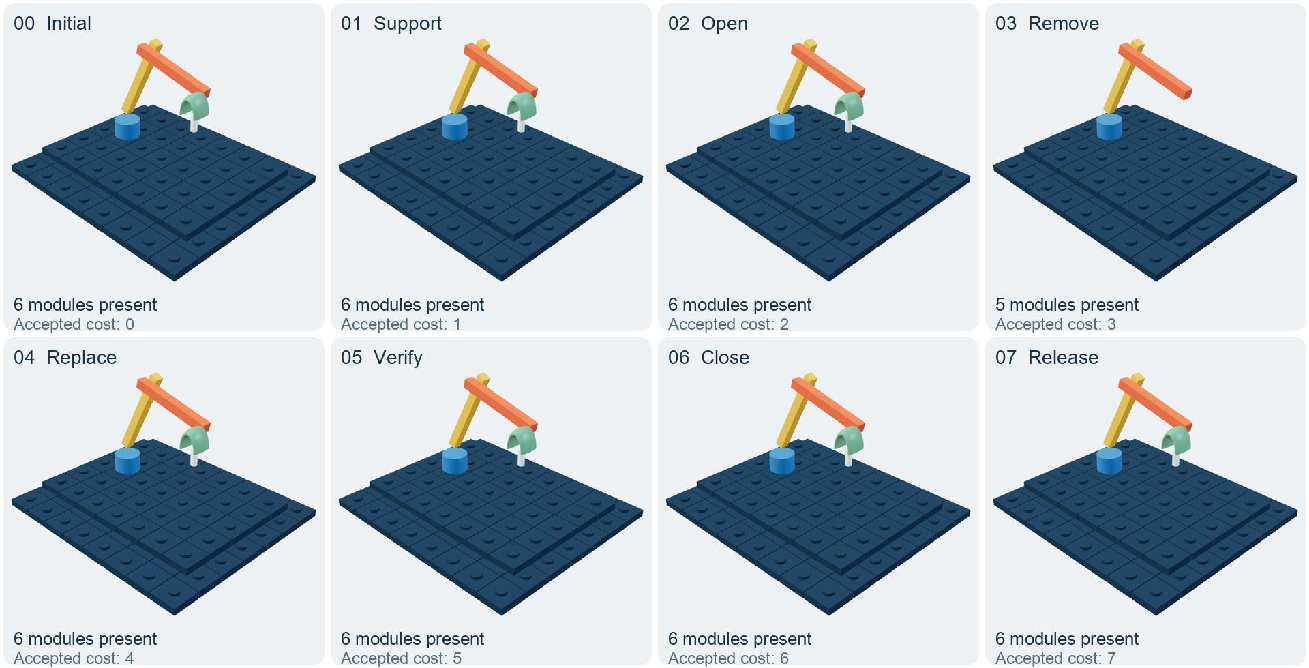
\includegraphics[width=\textwidth]{figures/publication-repair.pdf}
\caption{\textbf{Seven-step service repair on the same object.}
The tool disappears after removal and returns after replacement.
Support, access, verification, closure, and release update symbolic
facts; visually identical frames can therefore have different legal
next actions. Every frame is an actual replay state. The supplement
lists the exact facts and contrasts rejected removal attempts.}
\label{fig:repair}
\end{figure*}
Every configuration opens in the original application's 3D workspace
with orbit, zoom, pan, canonical views, module isolation, explosion,
and image export. Submitted or reference actions can be replayed
with a step slider and first-failure feedback. Selection and isolation
preserve the active modules at the selected frame.

Offline and website model records are byte-identical. The release
contains 576 canonical views, four per configuration. A review dashboard
supports per-task decisions, requires reasons for rejection, and
exports feedback for subsequent revision. This interface provides
review capability; it does not imply completed human annotation.
The supplement indexes every configuration and task family; full
inputs and answers are distributed in machine-readable records.

\section{Limitations}
The structural strata remain authored categories. No human timing
study, item-response calibration, or causal difficulty validation
has been completed. Shared constructors correlate layouts; 144
configurations do not represent 144 independent mechanical families.
The public development set and tiny historical pilot cannot establish
robust ranking, population accuracy, or generalization.

Physical realism is limited by compound bodies, cuboid envelopes,
anchored bases, and uncalibrated parameters. Declared graph edges
do not certify commercial connector compatibility. Symbolic repair
and exploded geometry are not collision-free robot trajectories.
Structured inputs may make many tasks solvable without images.
These limitations motivate family-disjoint hidden designs, manual
geometry review, calibrated connectors, human measurements, and
information-condition ablations.

\section{Conclusion}
BrickAtlas Hierarchy supports matched evaluation of brick structure,
reasoning, and executable intervention. Its 144 configurations and
48 repeated families provide 6,912 inspectable contracts, supported
by simulator records and 3D state replay. Data controls establish
execution consistency; independent model and physical validation
remain necessary to establish broader capability claims.

{\small\bibliographystyle{ieeenat_fullname}\bibliography{references}}
\end{document}
